\documentclass[12pt,a4paper,openany]{book}
\newcommand\tab[1][1cm]{\hspace*{#1}}
\usepackage{amsmath,amsthm,amssymb,graphicx,hyperref}
\usepackage[left=1.2in,right=1.2in,top=1in,bottom=1in]{geometry}
%\usepackage[romanian]{babel}
\usepackage[english]{babel}
\usepackage{xcolor}
\usepackage{paralist}
\RequirePackage{hyphenat}
\usepackage{algorithmic, algorithm}
\usepackage[inline]{enumitem}
\usepackage{fancyhdr}

\fancypagestyle{plain}{%
  \fancyhf{}% Clear header and footer
  \renewcommand{\headrulewidth}{0pt}% Remove header rule
}
%\setcounter{tocdepth}{3}
%\setcounter{secnumdepth}{3}

\newtheorem{thm}{Theorem}[section]
\newtheorem{lem}[thm]{Lemma}
\theoremstyle{definition}
\newtheorem{defn}{Definition}[section]
\theoremstyle{remark}
\newtheorem{rem}{Remark}[section]
\newtheorem{exmp}{Example}[section]

\title{BCI Applications Platform}
\author{Mihai-David Vuescu}



\begin{document}
\sloppy

\thispagestyle{empty}
\begin{center}
\begin{figure}[h!]
\vspace{-20pt}
\begin{center}

\includegraphics[width=100pt]{Graphics/FMI Logo.png}
\end{center}
\end{figure}


{\large{\bf WEST UNIVERSITY OF TIMI\c SOARA

FACULTY OF MATHEMATICS AND COMPUTER SCIENCE

BACHELOR STUDY PROGRAM:  Applied Computer Science}}

\vspace{120pt}
{\huge {\bf BACHELOR THESIS}}

\vspace{160pt}
\end{center}

{\large\noindent{\bf SUPERVISOR:
\hspace{172pt} GRADUATE: }

\noindent Conf. Dr. Cosmin Bonchis \hfill 
\noindent  Mihai-David Vuescu
}

\vfill
\begin{center}
{\bf TIMI\c SOARA

2023}
\end{center}
\newpage
\thispagestyle{empty}
\begin{center}
{\large{\bf WEST UNIVERSITY OF TIMI\c SOARA
		
FACULTY OF MATHEMATICS AND COMPUTER SCIENCE
		
BACHELOR STUDY PROGRAM:  Applied Computer Science}}

\vspace{200pt}
{\huge {\bf B.C.I. Applications Platform }}

\vspace{153pt}
\end{center}

{\large\noindent{\bf SUPERVISOR:\hfill GRADUATE:}

\noindent Conf. Dr. Cosmin Bonchis\hfill
\noindent Mihai-David Vuescu}
 

\vfill
\begin{center}
{\bf TIMI\c SOARA

2023}
\end{center}

% \newpage
% \normalsize{}


\tableofcontents
%%%%%%%%%%%%%%%%%%%%%%%%%%%%%%%%%%%%%%%%%%%%%%%%%
%%%%%%%%%%%% cap: Abstract %%%%%%%%%%%%%%%%%
%%%%%%%%%%%%%%%%%%%%%%%%%%%%%%%%%%%%%%%%%%%%%%%%%

\chapter*{Abstract}\label{cap:abstract_ro}
%%%%%%%%%%%% Section: Rezumat %%%%%%%%%%%%
Această lucrare de licență constă în realizarea unei platforme care interacționează cu o Interfață Creier-Calculator(ICC), mai exact cu interfața Unicorn Hybrid Black\cite{Unicorn_Technology}, pentru a facilita accesul la diverse aplicații compatibile. Scopul acestei platforme este de a face mai ușoară interacțiunea dintre o persoană cu dizabilități și un calculator în felul următor: de obicei când este nevoie de schimbarea aplicațiilor, utilizatorul cu dizabilități trebuie să aștepte după o altă persoană terță, fără dizabilități, care să schimbe aplicațiile și să recalibreze hardware-ul; prin crearea unei platforme care conține aplicațiile de care utilizatorul are nevoie și care îi permite aceluiași utilizator să schimbe de la un program la altul folosind o soluție deja existentă\cite{Unicorn_Speller}, nevoia de o astfel de persoană terță dispare, astfel dând utilizatorului libertatea de a folosi programele sale favorite fără să aibă nevoie de ajutor.
\vspace{\baselineskip}\newline
Având în vedere faptul că aplicația este destinată indivizilor cu dizabilități, va fi nevoie de asistență din partea unei persoane apte fizic pentru a adăuga noi aplicații pe platformă și pentru a elimina din cele existente în caz de nevoie. Pentru a ajuta în acest proces, o aplicație unealtă de tip installer a fost creată pentru a ajuta asistentul apt fizic în instalarea aplicațiilor ICC cu ajutorul unei interfețe grafice. Aplicațiile utilizate pentru a demonstra platforma vor fi preluate din aplicațiile create de studenții Universității de Vest Timișoara la hackathoanele br41n.io, în care aceștia au concurat cu aplicații care integrează interfețe ICC.
\vspace{\baselineskip}\newline
Astfel, această lucrare constă în două părți, soluția pentru realizarea platformei și soluția pentru realizarea aplicației pentru instalarea de aplicații noi. Pentru a crea platforma a fost folosit Unity engine pentru realizarea unei experiențe utilizator ușor de înțeles și pentru a crea legătura dintre aplicație și spellerul ICC proprietar Unicorn\cite{Unicorn_Speller} folosind limbajul de programare orientat obiect C\#. Aplicația tip installer este o aplicație dialog tip MFC scrisă în limbajul de programare C++ care se folosește de fișierele de tip batch pentru a descărca aplicațiile și pentru manipularea acestora în interiorul sistemului de fișiere Windows odată ce sunt descărcate. Deși ambele programe pot fi folosite separat unul de celălalt, folosirea acestora împreună creează o experiență mai ușoară pentru ambele categorii de utilizatori, atât cei cu dizabilități cât și cei apți fizic, astfel creând o soluție completă.


\chapter*{Abstract}\label{cap:abstract_en}
%%%%%%%%%%%% Section: Abstract %%%%%%%%%%%%
This bachelor's work consists in realising a platform that works in conjunction with a Brain-Computer Interface(BCI), specifically the Unicorn Hybrid Black BCI\cite{Unicorn_Technology}, to facilitate access to applications compatible with the aforementioned platform. The platform aims to improve accessibility for a disabled person that is using a BCI as follows: normally when changing between applications the disabled subject must wait for an able-bodied helper to change applications and recalibrate the hardware; by creating a platform that houses applications the user may need and that allows the user to change between them seamlessly using an already existing solution\cite{Unicorn_Speller} the need for the said helper is removed, thus giving the end-user more freedom in interacting with his/her favourite programs. 
\vspace{\baselineskip}\newline
Due to the fact that the application is targeted at impaired individuals, the need for an able-bodied helper will arise when it comes to adding new applications to the platform and/or removing existing ones should that need to arise. An installer tool was created to aid the helper in installing the BCI applications via a graphical user interface. The apps used to demonstrate the platform will be taken (with permission) from UVT's submissions in the br41n.io hackathons, in which students competed with ideas for applications that integrate Brain-Computer interfacing.
\vspace{\baselineskip}\newline
Accordingly, this paper consists of two main parts, the platform solution itself and the installer solution. In creating the platform, the Unity engine was employed for creating an easy-to-understand user experience and for interfacing with Unicorn's proprietary BCI speller\cite{Unicorn_Speller} using the C\# programming language. The installer tool is an MFC-type dialogue application written in the C++ programming language that uses batch files to download and manipulate the application files inside of the Windows file system. While both programs can be used separately, they create an easier user experience for both user groups if used together: the impaired and the helpers, consequently creating a complete solution.

%%%%%%%%%%%%%%%%%%%%%%%%%%%%%%%%%%%%%%%%%%%%%%%%%
%%%%%%%%%%%% cap: intro %%%%%%%%%%%%%%%%%
%%%%%%%%%%%%%%%%%%%%%%%%%%%%%%%%%%%%%%%%%%%%%%%%%
\pagestyle{fancy}
\fancyhf{}% Clear header and footer
\fancyhead[RO,LE]{\thepage}% Page number on the outer (RO/LE) side of the header
\fancyhead[RE]{\nouppercase{\leftmark}}% Section name on the inner (RE) side of the header
\renewcommand{\headrulewidth}{0pt}% Remove header rule


\chapter{Introduction}\label{cap:intro}



%%%%%%%%%%%%%%%%%%%%%%%%%%%%%%%%%%%%%%%%%%%%%
%%%%%%%%%%%% Section: Motivation %%%%%%%%%%%%
%%%%%%%%%%%%%%%%%%%%%%%%%%%%%%%%%%%%%%%%%%%%%
\section{Project Motivation}\label{sect:motivation}
This project started from a wish to create a platform to store all BCI applications developed by the University's(West University of Timișoara) BCI teams during hackathons and other contests. Being part of said teams, it became apparent that most of the aforementioned applications could not be operated by a person with disabilities.
\vspace{\baselineskip}\newline
There are numerous applications developed for BCI systems, with some believing them to be the future of entertainment and the next step beyond AR and VR for an able-bodied user\cite{future_of_metaverse_BCI}. That leaves a lot to be desired when it comes to the initial purpose of the BCI, which was to be a prosthetic for the brain, with the focus being on disabled people. The research for BCIs has come a long way since the first experiments which were performed on primates in the late 60s\cite{Fetz_1969}, with modern BCIs being used for both medical purposes and entertainment. 
\vspace{\baselineskip}\newline
As such, numerous applications are being developed for BCI users. The applications are however disconnected from one another such as the end-users would have a hard time adjusting from one to the other on their own. This is a major problem since the end-user is more often than not a disabled person requiring a helper. By creating this platform application I wanted to bridge the gap between applications and disabled users while taking advantage of the lack of consumer solutions when it comes to housing multiple applications in one place. I chose this topic for my bachelor's thesis in the hopes of creating such an application and in the hopes of making it easier for a disabled person to do the thing I loved doing all my life: using a computer.



%%%%%%%%%%%%%%%%%%%%%%%%%%%%%%%%%%%%%%%%%%%%%
%%%%%%%%%%%% Section: Objectives %%%%%%%%%%%%
%%%%%%%%%%%%%%%%%%%%%%%%%%%%%%%%%%%%%%%%%%%%%
\section{Objectives}\label{sect:objectives}
From a general standpoint, the main objective of the platform is described in the above section of this paper: making a cohesive application that integrates with a well-known BCI speller to deliver seamless access to different apps for a disabled user. The platform should be intuitive and easy to use, such as no explanations should be needed before using the platform. 
\vspace{\baselineskip}\newline 
From a technical standpoint, this project aims to create a stable system capable of housing a considerable quantity of applications without failure. Due to the platform relying on multiple components (the speller, the individual applications, the speller receiver, and the platform logic itself), multiple points of failure exist. In the case of an unhandled crash, an able-bodied helper is once again needed, thus defeating the general purpose of the app. As such, error handling inside the application is the priority. 
\vspace{\baselineskip}\newline
When it comes to compatibility, the objective is to make apps integrate with the platform. This requires modifying the apps to be contained inside the platform to make them compatible. To reach this objective without compromising the aforementioned two, the platform will require as little tinkering on the application side as possible, ensuring that adding a new application is as easy as dragging and dropping its folder into the platform's own. The installation of new applications within the platform will fall into the hands of an able-bodied person, this is one of the limitations of the platform. 
\vspace{\baselineskip}\newline
All objectives hinge on the experience of the end-user and all features of this project are catered towards a disabled individual. This solution tries to prioritize accessibility and ease of use over other aspects. That being said, no testers from the target demographic have been employed in developing this solution, so it may or may not work as intended on the targeted user base. That being said, the implementation method may also work on other problems that require a platform controlled by the user.
\vspace{\baselineskip}\newline
Therefore we can conclude with 3 primary objectives: creating an easily understandable and navigable user experience, ensuring the stability of the proposed solution, and developing a way to integrate apps within the platform without the need to modify the apps themselves to fit in.



%%%%%%%%%%%%%%%%%%%%%%%%%%%%%%%%%%%%%%%%%%%%%%%%%%%%
%%%%%%%%%%%% Section: Similar Solutions %%%%%%%%%%%%
%%%%%%%%%%%%%%%%%%%%%%%%%%%%%%%%%%%%%%%%%%%%%%%%%%%%
\section{Similar Solutions}\label{sect:similar solutions}

\subsection{Unicorn Suite}
The best example of an application platform is the one that will be used in realising this thesis, the Unicorn Suite Hybrid Black. Inside the Suite, there are different applications created by g.tec, such as the Unicorn Recorder, Bandpower and UDP Interface among others, as well as different APIs intended as a means of integration with different applications. All of the said applications can be accessed through the suite, with some being behind a paywall while others being readily available as soon as the user downloads the suite\cite{Unicorn_Suite}. This solution is a notable system with high versatility and compatibility with various software solutions developed by g.tec to aid in using the Unicorn BCI.

\subsection{BCI2000}
BCI2000 is an open-source software system for BCI research that is free for any non-commercial use. The system includes software tools that can acquire and process data, present stimuli and feedback and manage the interaction with different outside devices such as robotic arms. BCI2000 is real-time, having the ability to synchronise EEG and other signals with a wide variety of biosignals and input devices such as computer mice or eye trackers. It has several modules to manage data importing and exporting in common file formats. BCI2000 operates on most Windows systems and the source code can be compiled on most Windows machines\cite{BCI2000}. The BCI2000 has different tools for users and developers, with numerous resources such as tutorials and references for further research. There are also multiple publications associated with BCI2000. Overall, the general-purpose platform created by BCI2000 is flexible and can integrate many different applications.

\subsection{OpenViBE}
OpenViBE is an open-source software platform dedicated to designing, testing and using BCIs. It is described as being software for real-time neurosciences (real-time processing of brain signals) which can be used to acquire, filter, process, classify and visualise brain signals in real-time. Since version 2.2.0, OpenViBE includes tools for offline and batch analysis of large datasets. The main use cases for OpenViBE are the medical field (assistance to disabled people, real-time biofeedback, neurofeedback, real-time diagnosis), multimedia (video games, VR), robotics and other fields related to brain-computer interfacing.

\subsection{Others}
Other platforms and systems housing BCI tools exist. Research papers such as BCI Software Platforms(Brunner et al., 2012) list 7 publicly available software platforms for brain-computer interfaces, as well as possible synergies and future developments, such as combining different components of different platforms\cite{Brunner_2012}. Other papers such as Research of Auxiliary Game Platform Based on BCI Technology(Jiang et al., 2009) present a solution for controlling video games by BCI using motor imagery, translating the motor imagery EEG into three control signals: left, right or stop; a simple game player can use it as an input device of to realise the function of operating games\cite{Jiang_2009}.
\vspace{\baselineskip}\newline
As the field of brain-computer interfacing alongside other related fields such as neuroscience, biomedical engineering and computer science advance, more solutions will be available for the public at large to experiment with. Within 60 years, the field has moved from simple artefact-sensitive EEG to making real the vision of brain-computer communication, resulting in long-term at-home usage for patients with locked-in syndrome\cite{K_bler_2019}. More innovation will bring different new implementations and similar solutions, as BCI as an assistive technology will likely be perceived as an integral part of life in the decades to come\cite{K_bler_2019}.

\newpage

%%%%%%%%%%%%%%%%%%%%%%%%%%%%%%%%%%%%%%%%%%%%%%%%%%%%
%%%%%%%%%%%% Section: Similar Solutions %%%%%%%%%%%%
%%%%%%%%%%%%%%%%%%%%%%%%%%%%%%%%%%%%%%%%%%%%%%%%%%%%
\section{Scope of Contribution}\label{sect:Scope of Contribution}

This section aims to outline my contributions to the works already existing at the time of writing the present work. This is necessary because the platform created as a result of this work is based on closed-source software to which I had no contribution and which I did not and could not modify. In this section, I will not mention the hardware used as none of it is of my making, instead being built and tested by g.tec Austria.


\subsection{Foundational Works}
First and foremost, the foundation upon which the platform is based is the Unicorn Software Suite, specifically the Unicorn Speller. None of the code inside the speller is my own. I did not modify any of the code because the Unicorn software is closed-source. Furthermore, the data transfer methods, such as protocols and data formats are not my own as they are part of the Suite. I only parsed the data that was sent by the hardware and used the Speller as an input method to the platform.
\vspace{\baselineskip}\newline
When it comes to the applications used inside of the platform, they were coded and built by several teams from the West University of Timișoara during hackathons and other BCI competitions. I was part of some of the teams, but I cannot claim ownership of any application since creating them was a team effort and the application ownership is that of the teams themselves and not particular members. The applications themselves are detailed in section \ref{sect:Applications Used}.
\vspace{\baselineskip}\newline
To conclude foundational works, I want to touch on the plethora of research and papers used throughout this paper. None of the research mentioned or cited is my own and specific authors are listed in the bibliography section of this paper [see bib. \ref{sec:bibliography}]. The field of BCIs has seen a boom in popularity and research. Since 2019 there have been over 22,000 published papers about or related to Brain-Computer Interfacing\cite{bci_scholarly_articles}. While the theory in regards to the field of BCI may be lacklustre at times throughout this paper, this is necessary to ensure the information is digestible and on the topic of the project at hand. For any further reading, refer to the bibliography of this paper. Moreover, this paper doesn't bring any new academic research to the table but builds on existing research.


\subsection{Personal Contributions}
My contribution to the subject at hand begins with the platform itself. I created the graphical user interface and wrote the logic behind it. I created the system for downloading and installing applications from Git Hub using the installer mentioned in this paper [see chapter \ref{cap:installer}] and programmed the platform to detect applications loaded using the install wizard or applications placed manually inside the platform app directory.
\vspace{\baselineskip}\newline
Using the Unicorn Speller and its executable file, I created a method for loading speller boards dynamically based on which application is opened to maximise compatibility with applications made by other users [see subsect. \ref{subsect:Board Change}].
\vspace{\baselineskip}\newline
One of the problems encountered during the making of the platform was UDP port binding and locking out input. To pass input from the platform to the application, I created a UDP relay [see sect. \ref{sect:UDP Relay}] inside the UDP listener so that the platform takes input first, parses it and then passes it forward to the open application.
\vspace{\baselineskip}\newline
As of my research at the time of writing this paper, there are no other BCI platforms for user-created applications, or at least no public ones readily available on the internet for the hardware used in this paper (the Unicorn BCI). By creating an open-sourced solution available for anyone to download, anybody can use it in different contexts. As it stands, g.tec's software is fairly rigid, not allowing hot-swapping boards and using multiple applications at once. In the making of the present solution, I remediated this issue and created a flexible solution in its place using Unicorn software.


%%%%%%%%%%%%%%%%%%%%%%%%%%%%%%%%%%%%%%%%%%%%%%%%%
%%%%%%%%%%%% cap: theory %%%%%%%%%%%%%%%%%
%%%%%%%%%%%%%%%%%%%%%%%%%%%%%%%%%%%%%%%%%%%%%%%%%

\chapter{Theoretical Basis}\label{cap:theory}
To fully understand this paper and the development of its proposed solution, it is necessary to first understand some basic concepts and the theory regarding the current context. The purpose of this second chapter is to describe and explain notions regarding the subject at hand and to give examples of how they fit into the proposed solution.


%%%%%%%%%%%%%%%%%%%%%%%%%%%%%%%%%%%%%%%%%%%%%
%%%%%%%%%%%% Section: Neurotechs %%%%%%%%%%%%
%%%%%%%%%%%%%%%%%%%%%%%%%%%%%%%%%%%%%%%%%%%%%
\section{Neurotechnology}
\subsection{Electroencephalography (EEG)}
Electroencephalography or EEG is a method of recording an electrogram of the brain's spontaneous electrical activity. Brain cells communicate via electrical impulses and are active all the time, even during sleep\cite{EEG_mayoclinic}. This activity shows up as wavy lines on an EEG recording[see Fig 2.1]. For the purpose of realising this thesis I am using a non-invasive EEG method via the electrodes provided with the Unicorn Hybrid Black BCI[see fig 2.2].

\begin{figure}[H]
    \begin{minipage}[c]{0.45\linewidth}
      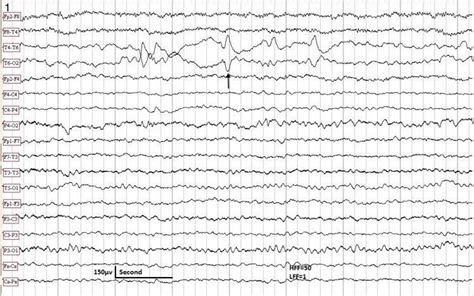
\includegraphics[width=\linewidth]{Graphics/EEG Example.jpeg}
      \caption{Sample EEG}
      \end{minipage}
    \hfill
    \begin{minipage}[c]{0.45\linewidth}
      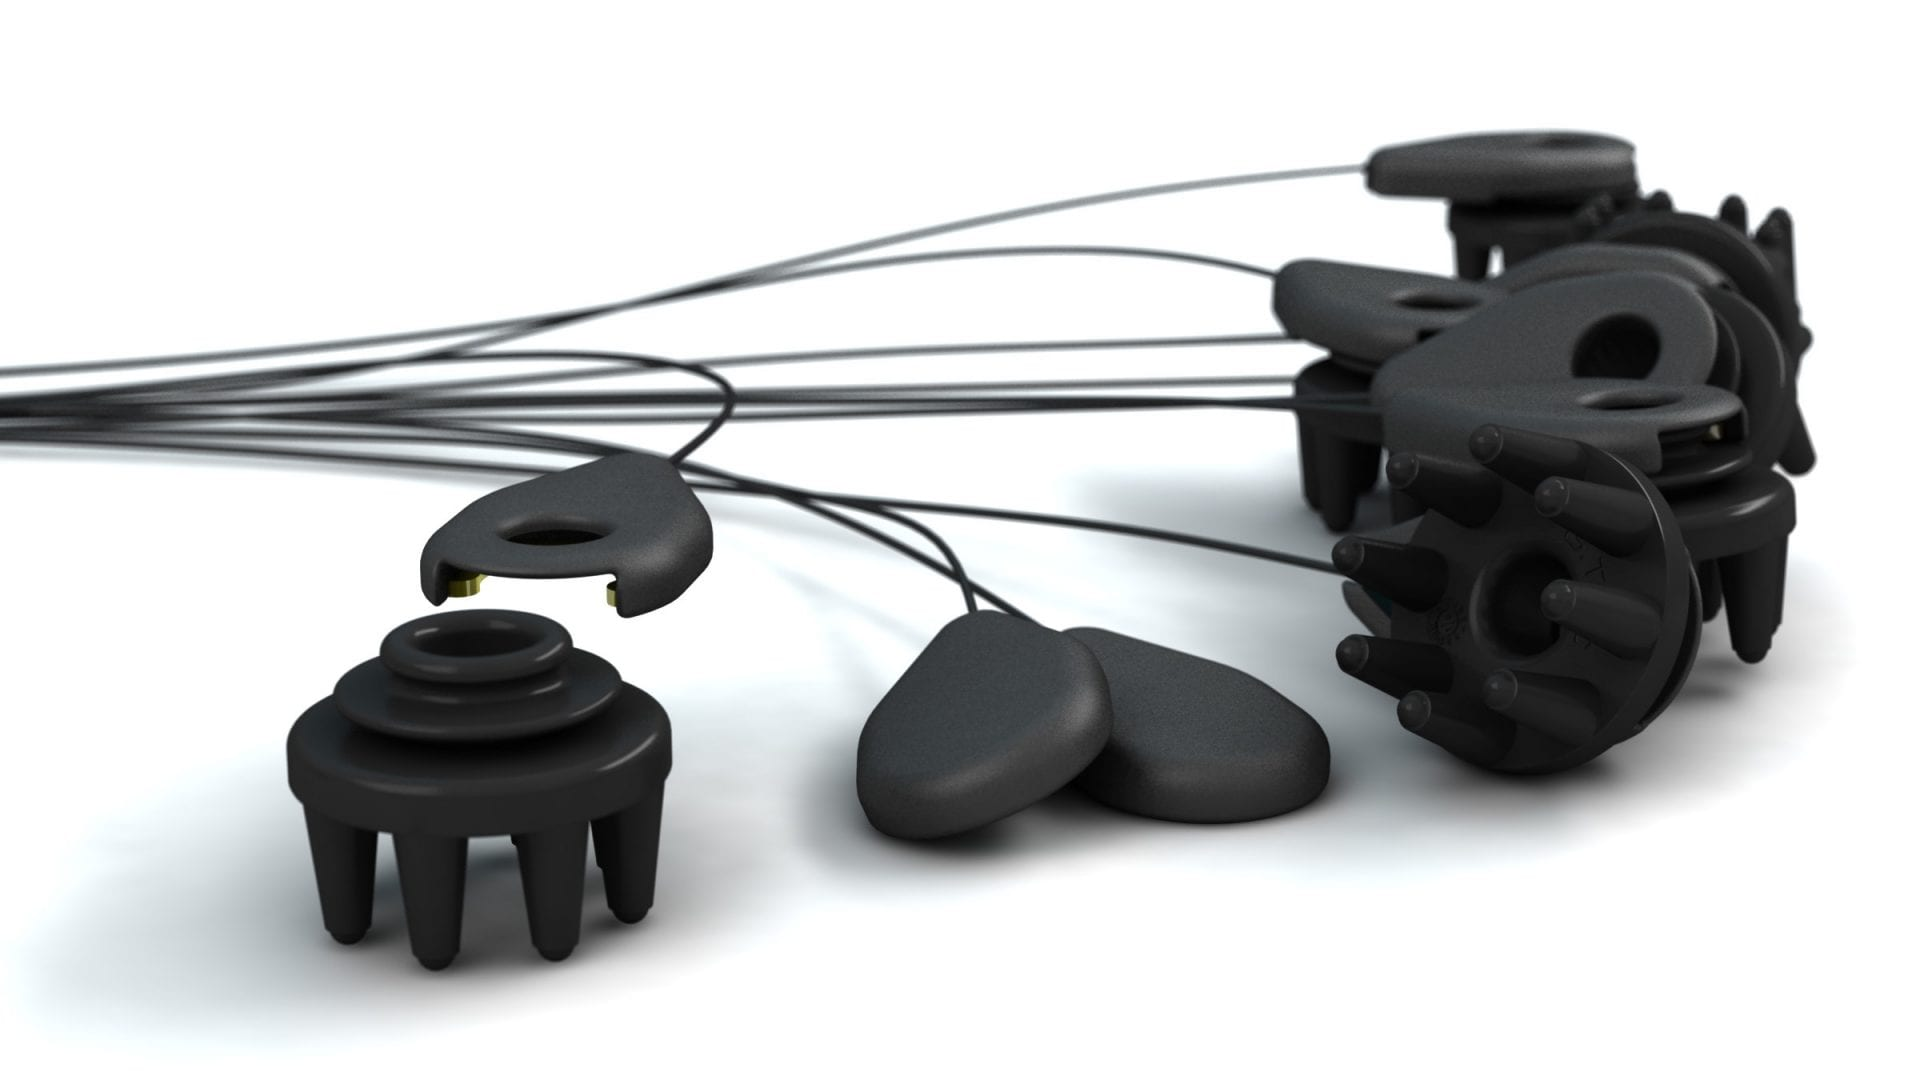
\includegraphics[width=\linewidth]{Graphics/Unicorn Electrodes.jpg}
      \caption{Unicorn Electrodes}
  \end{minipage}%
\end{figure}

Non-invasive EEG methods measure voltage fluctuations at the scalp which are produced by neuronal activity in the brain, but it is difficult to trace these signals back to the brain. As such, EEGs have low special resolution and are unable to provide precise information. Coupled with signal noise from various sources (electrical interference, muscle activity, eye movements, etc.) and interference from the skin and the skull, this makes the EEG a very sensitive tool. This can make results vary greatly, with the same user sometimes generating different results in the same testing medium. The signals may also get weaker and less accurate over time due to the user's state of mind and body (level of alertness, mental fatigue, physical fatigue, etc.) and the user may move the electrodes involuntarily as they are in use through normal body movement. There is also a case to be made about the comfort of the user which can play a vital role in getting the best results, as an uncomfortable user will pay less attention to the task at hand and thus generate more noise, inaccuracies and instability in an already sensitive system.


\subsection{P300}
The P300 is a component of event-related potential (ERP) used in decision-making. It is used in measuring the user's reaction to an external stimulus. It is implemented using the Oddball Paradigm, an experimental design in psychological research, where the stimulus to be observed is introduced between other redundant stimuli.

\subsection{Brain-Computer Interfacing}
A brain-computer interface(BCI) or brain-machine interface(BMI) is a computer-based system that acquires brain signals, analyses them and translates them into usable data or commands which are then exported to other devices to be used to other extents. By definition, a BCI uses some form or another of data processing and as such an EEG alone cannot be called a BCI\cite{Shih_2012}. BCI implementations vary based on the invasiveness of their data acquisition methods. As such, there are non-invasive BCIs (using electroencephalography, magnetoencephalography, electrooculography or magnetic resonance imaging), semi-invasive BCIs (using electrocorticography and endovascular methods) and invasive BCIs (using microelectrode arrays).

\subsection{Unicorn Hybrid Black BCI}
The BCI that will be used in the implementation of this paper is the Unicorn Hybrid Black. This is a non-invasive BCI using EEG technology. The 8 electroencephalogram electrodes are placed at the following fixed positions on the provided cap: Fz, C3, Cz, C4, Pz, PO7, Oz and PO8[see fig 2.3], in accordance with the 10/20 international system. Two extra electrodes marked L and R are to be attached to the mastoid bones behind the user's ears and act as a "ground" for the rest of the electrodes due to their placement on an area with virtually no electrical activity. 

\begin{figure}[H]
  \centering
  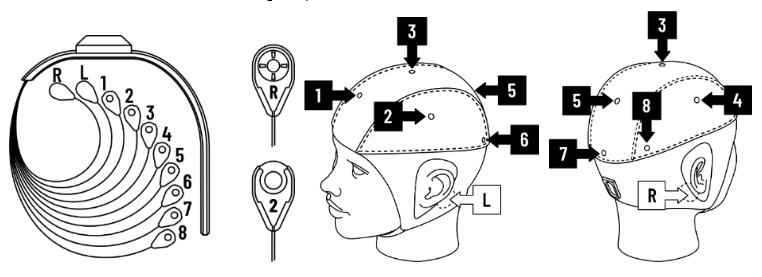
\includegraphics[width=0.8\textwidth]{Graphics/Electrode Placement.png}
  \caption{Electrode placement on the cap}
\end{figure}

The EEG cap works with 8 channels(with 2 extra "ground" channels) on a 24-bit resolution and a refresh rate of 250 hertz. The data is outputted via Bluetooth to a computer where it is processed.


%%%%%%%%%%%%%%%%%%%%%%%%%%%%%%%%%%%%%%%%%%%%%
%%%%%%%%%%%% Section: Techs %%%%%%%%%%%%%%%%%
%%%%%%%%%%%%%%%%%%%%%%%%%%%%%%%%%%%%%%%%%%%%%
\section{Technologies Used}
\subsection{Unicorn Suite}
The Unicorn BCI always comes alongside the Unicorn Suite, a software environment touched upon in the similar solutions section of this paper. In this implementation, the suite is used for its development tools and the Unicorn Speller contained within. Other useful tools include the Unicorn recorder, the .NET framework which uses the C\# programming language and other tools that allow the creation of different software solutions. Another function of the Suite is to keep the licenses required to use the software, as most tools require licenses purchased directly from g.tec\cite{Unicorn_Shop}, including the Speller used in this implementation.


\subsection{Unicorn Speller}
The Unicorn Speller is a spelling system that uses the P300 complex\cite{UnicornSuite_Manual}. The speller's interface consists of a QWERTY key layout that sits on the screen along a number row, an auto-complete row and a special functions row[see Fig 2.4]. The numbers and letters are used for spelling while the special keys are used for other functions such as text-to-speech, printing, etc. Each key is considered an item, and the layout is called a board. The user can choose the board he/she wants to use, thus choosing the layout of the items on the screen. The speller also allows for the creation of user-made boards (using the \textit{.ibc} file extension), the use of which will also be employed in this work. 
\vspace{\baselineskip}\newline
The actual mode of operation of the speller is through "flashing"\cite{UnicornSuite_Manual}, where the items on the board are flashing a different image for a brief moment (eg. the letter S is replaced with the face of Chuck Norris for a brief second before returning to its normal appearance). The images that flash on the letters are usually the faces of famous people. This is due to discoveries regarding P300 spellers, where researchers found out that superimposing familiar faces on letters helps accuracy and improves the performance of the ERP\cite{Li_2015}\cite{Kaufmann_2011}. To select an item, the user must focus on said item and count each time the item he/she wants to select flashes and ignore all other flashes\cite{UnicornSuite_Manual}.

\begin{figure}[H]
  \centering
  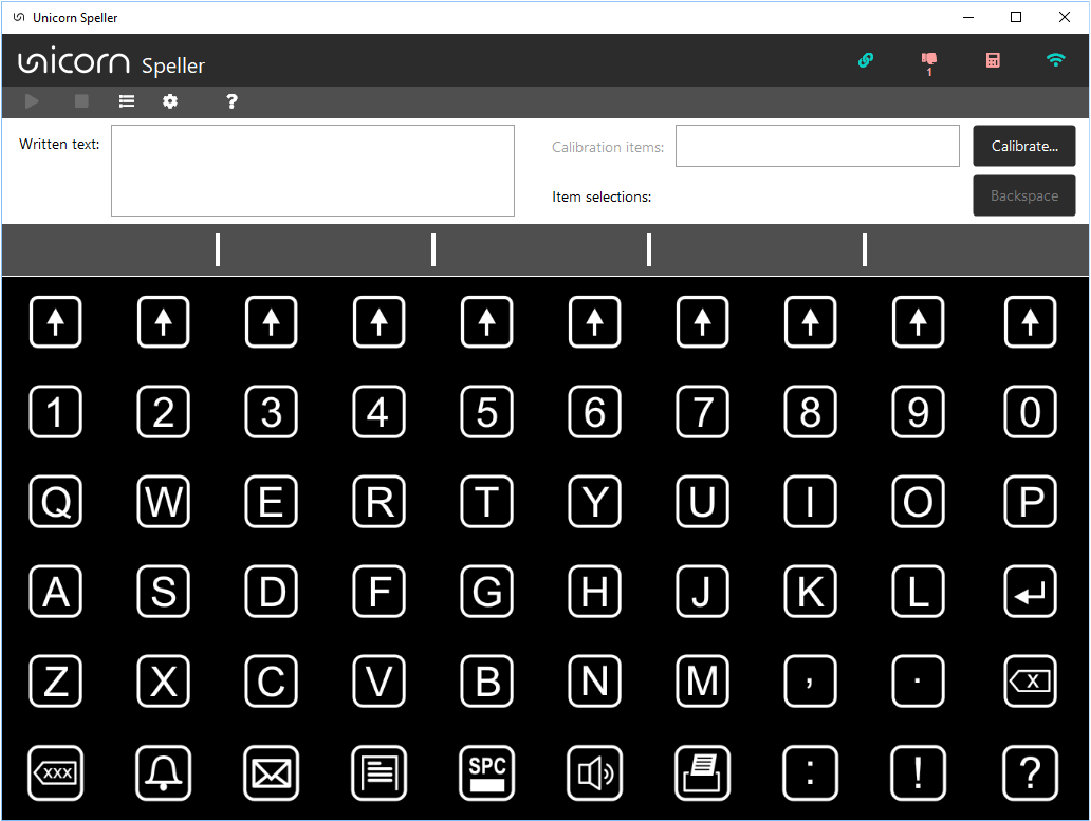
\includegraphics[width=1\textwidth]{Graphics/Speller.png}
  \caption{Unicorn speller using the default board}
\end{figure}

The speller flashing occurs in flash cycles, a group of flashes such as that each item on the board has flashed exactly once. There are different modes of flashing that the user can choose from as follows: row/column, single character and randomised patterns. To create the solution proposed by this paper, I will be using the randomised patterns mode, a randomised selection of items distributed across the whole board that flash at the same time, with patterns flashing consecutively\cite{UnicornSuite_Manual}. 
\vspace{\baselineskip}\newline
Furthermore, to use the speller, a calibration sequence needs to be completed. To calibrate, we must input a word or different letters that the user has to look at while the calibration sequence runs[see Fig 2.4]. During calibration, the speller learns the difference between the user's typical EEG signals and afterwards, it creates a calibration file, storing the user's calibration data to be reused. In this way, the speller adapts to the user, each user having different calibrations depending on different variables such as the user's environment. Therefore, it is best to calibrate in a quiet place, away from distractions and disturbances that might introduce rubbish data and noise in the calibration file.

\begin{figure}[H]
  \centering
  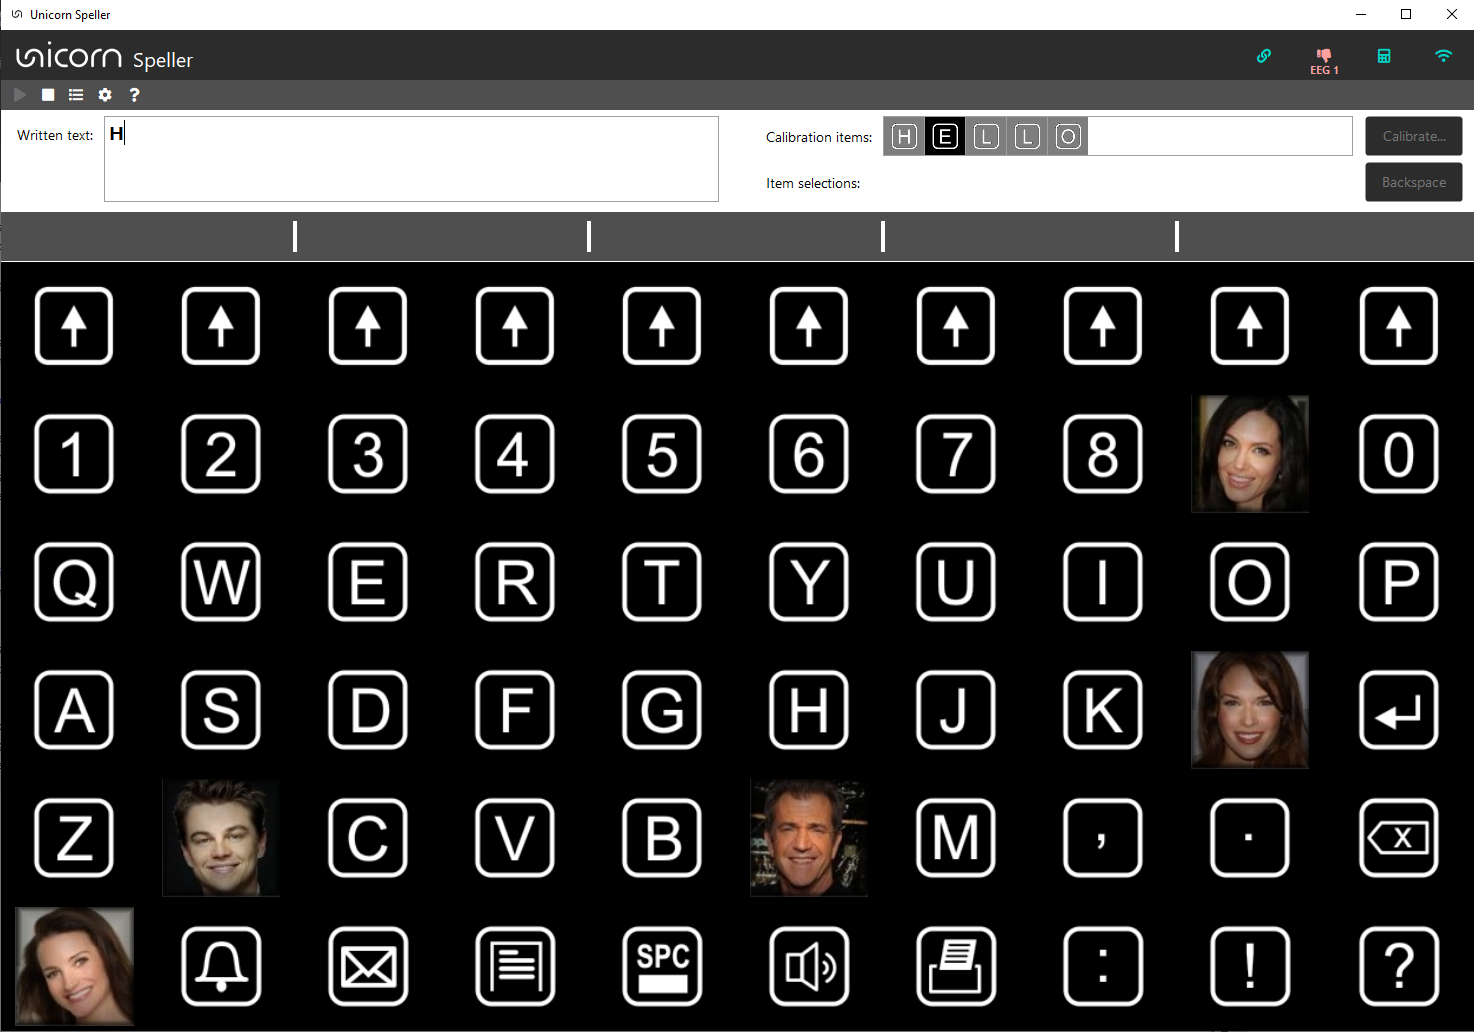
\includegraphics[width=1\textwidth]{Graphics/Speller Calibration.png}
  \caption{Calibration sequence}
\end{figure}
\vspace{\baselineskip}


\subsection{Unity Game Engine}
The Unity engine is a game development platform created by Unity Technologies which offers multiple solutions for creating both 2D and 3D applications and games. Used in multiple fields such as the automotive industry, engineering and architecture\cite{Unity_engine}, the platform is an easy and intuitive way to create different software implementations. Furthermore, the engine supports cross-platform deployment of applications, making it facile to distribute software solutions without hassle. This feature will however not be taken advantage of in the execution of this work, because the unicorn software doesn't work on UNIX-based systems\cite{UnicornSuite_Manual}.
\vspace{\baselineskip}


\subsection{Visual Studio 2022 IDE}
Visual Studio 2022 is an Integrated Development Environment (IDE) used for editing, debugging, building code and publishing different applications. Visual Studio includes compilers, code completion tools, graphical designers and other features to enhance software development processes\cite{VisualStudio}. Visual Studio also provides plugins and different integration with external tools, such as the Unity Game Engine. In the making of this bachelor's work, the main Development Environment used is the 2022 version of this IDE, both as the default script editor for Unity and in other miscellaneous tasks as a code editor.
\vspace{\baselineskip}\newline
Due to the comprehensive support for Microsoft Foundation Class (MFC) applications, the IDE was also used to create the platform's installer, which is an MFC-type application. Visual Studio has extensive tools for designing the MFC user interface and the logic behind it and was crucial in developing, building, running and deploying the platform's installer.
\vspace{\baselineskip}\newline
For trivial and smaller code editing tasks, the simpler Visual Studio Code was used as a quicker alternative to the vastness of its bigger and more complex counterpart.
\vspace{\baselineskip}\newline


\subsection{Programming Languages Used}
\subsubsection{C\#}
C\# is a modern, innovative, open source and multi-platform Object-Oriented Programming (OOP) language\cite{C_sharp} developed by Microsoft. C\# is one of the top 5 languages used by projects on GitHub and one of the most loved languages on Stack Overflow\cite{StackOverflow_language_survey}. The language is a high-level programming language, featuring garbage collection for better memory management. It is also the primary language used for scripting in the Unity game engine. Inside the engine, the language is used to create scripts that control app behaviour by attaching said scripts to in-engine objects to control their behaviour. They can also be used to control global application properties inside Unity. As such, it is the main language used in creating the graphical user interface of the platform and it is also used for creating the speller receiver, a script that asynchronously awaits input from the Unicorn BCI.

\subsubsection{Visual C++}
Visual C++ is a programming language and development environment provided by Microsoft which is a version of the C++ language with added support for Windows-based development. Visual C++ is part of the Visual Studio IDE, making the development process much easier through the use of the powerful IDE's tools. The language also has .NET support, making the use of .NET libraries possible. Its compiler is also highly capable, being able to generate highly optimised machine code for the Windows platform.

\subsubsection{Batch Scripting}
While not a programming language, batch scripting consists of a series of commands that are then executed on a line-by-line basis by the shell program (in this case cmd.exe). Batch files are used to simplify routine and repetitive tasks. A file of this type is an unformatted text file that consists of one or more commands bearing the file extension \textit{.bat} or \textit{.cmd}. After a run, the batch file returns a value of 0 if the run went smoothly or a value of 1 if errors occurred during the execution of the batch file\cite{batch_files}. In this project, batch files are used inside the installer tool application to execute system calls, move apps across the file system and send requests to GitHub.
\vspace{\baselineskip}\newline


\subsection{GitHub}
GitHub is a hosting platform for version control and collaboration\cite{github_HelloWorlds}. It was founded on Git, an open-source code management system created by Linus Torvalds. Git is widely used in the programming community for storing code and tracking the history of said code from its inception. Another key feature is collaboration, with Git allowing developers to collaborate on a project, providing code conflict resolution tools. GitHub provides a web interface for the Git code repository alongside other collaboration and management tools\cite{whatsGithub}. During the development of this thesis, GitHub was used as a versioning system for the platform application, the installer application and the LaTeX thesis, the present document, itself.
\vspace{\baselineskip}\newline
Alongside the present bachelor's work, all the BCI applications developed by me and my colleagues during our Bachelor's degree at the West University of Timisoara are also stored and versioned on the website. The release feature on the website is used to store binary files containing executables for easy downloading, with each application having its own release. Using the GitHub API to send requests to the platform, the aforementioned binaries can be downloaded from the command line. This is the mechanism that stands behind the installer tool, making it possible to grab all applications at once and store them on the user's computer.


%%%%%%%%%%%%%%%%%%%%%%%%%%%%%%%%%%%%%%%%%%%%%%%%%
%%%%%%%%%%%% cap: features %%%%%%%%%%%%%%%%%
%%%%%%%%%%%%%%%%%%%%%%%%%%%%%%%%%%%%%%%%%%%%%%%%%

\chapter{Application Features}\label{cap:features}

%%%%%%%%%%%% Section: Features %%%%%%%%%%%%
\section{Features}\label{sect:features}
\textbf{Seamless integration with Unicorn Hybrid Black}. The application will be designed to work with gTec's unicorn technology seamlessly. The end user will only have to configure the BCI for the specific end-user and afterwards everything is smooth sailing.

\vspace*{2mm}
\textbf{Friendly Dynamic UI}. The platform itself will have an easy to navigate graphical user interface for both the BCI user and the helper. The platform will also be able to refresh to accomodate newly added and/or freshly deleted applications. This way. This way, no lousy restarts of the whole application will be needed to make the platform show new applications. This also works well in limiting errors, since deleted applications will dissapear entirely, making it impossible for the BCI user to select an application that isn't there anymore.

\vspace*{2mm}
\textbf{Drag and drop}. Adding new applications and deleting existing ones should be as easy as dragging and dropping the application in the apps folder or deleting an existing app. The platform can recognise this and adapt accordingly.

\vspace*{2mm}
\textbf{Helper button}. If the BCI user wishes to call the helper, the platform can facilitate that via a button that alerts the user's caretaker using noise.

\newpage


%%%%%%%%%%%% Section: Features %%%%%%%%%%%%
\section{Implementation Details}\label{sect:implement_details}
\textbf{Visual C\#}. The GUI is built using visual C\#. This is to ensure stability and an easy way to add new features down the line. Different styles are also used to make the interface visually appealing to the end-user.

\vspace*{2mm}
\textbf{Local app storage}. The different applications are stored locally. This makes it easier for the user's helper to add and remove them when the need arises.

\vspace*{2mm}
\textbf{Unicorn Speller}. The app makes use of the pre-existing unicorn speller software with a custom board made for the application platform. The speller board gives the BCI user all necessary input while using the application and is initialised when the application starts.

\vspace*{2mm}
\textbf{UDP port listener}. To ensure communication between the platform itself and the unicorn speller, the two major components of this bachelor's work, a UDP listener is implemented in the platform logic. The listener awaits for input from the speller on a specific port and once it receives it sends the signal further along to the platform which reacts accordingly. Once an application is open, it uses its own means of listening to the user input.

\bibliography{bibliography}
\bibliographystyle{unsrt}
\addcontentsline{toc}{chapter}{Bibliography}

\end{document} 
